\documentclass{article}
\usepackage[utf8]{inputenc}
\usepackage{graphicx}
\graphicspath{ {images/} }
\usepackage{url}
\title{How Social is Imgur?\\Mapping and Analyzing the Connectivity of the Community}
\author{Jon Rusert}
\date{December 2017}

\begin{document}

\maketitle

\section{Imgur}
\par Imgur.com is an online image sharing site. The website currently reaches over 250 million people each month while boasting billions of image post views each month\cite{imgurabout}. Imgur is also currently ranked as the 13th most popular website in the United States according to
Alexa\cite{alexa}. We will briefly visit the history of Imgur, then show why the Imgur community poses an interesting format for graph analysis.

\subsection{History of Imgur}
Imgur was created in 2009 by Alan Schaaf as an image hosting site for the text based website Reddit\cite{imgurabout}. In 2010, users are able to create accounts and the "Gallery" is created which showcases the most popular images on the website. Starting in October 2012, Imgur users are given the ability to submit images directly on the website (aptly named User Submitted) to be shared directly with the Imgur community and not necessarily with other websites (such as Reddit). In 2013, Imgur reaches over 100 million monthly active users, then reaches over 150 million people per month in 2015, while currently reaching over 250 million people per month in 2017. 
\par As can be seen, the Imgur community continues to steadily grow. As the community has grown it has also evolved into an nontraditional social community.

\subsection{Imgur Community}\label{community}
\par Although users are able to create accounts, currently there are no prominent social connections between users. Many other social media websites, (i.e. Facebook, Twitter, Instagram, etc.), include a way to stay in frequent observable contact with other users. Facebook includes having friends, while Facebook, Twitter, and Instagram all allow users to "follow" each other and observe their daily activities. Imgur does not have either friends nor followers. Instead, the observable interactions are done on the images being hosted themselves. These interactions include posting an imgae to Imgur, upvoting/downvoting images/comments on the images, commenting on the posted image, and replying to comments. The users you interact with generally are thought to change from image to image. 
\par While it appears from the outside that no observable community exists within Imgur, Imgur has demonstrated the existence of the community through several community events. One such event is "Imgur Secret Santa". Imgur Secret Santa entails users volunteering to send Christmas gifts to other users all across the United States, as well as international gift giving. Over 33,000 users registered for the most recent Imgur Secret Santa\cite{gag}. Another community event which occurred was "Camp Imgur". Camp Imgur was an event organized by the staff of Imgur in 2015 to host a large meet up of Imgur users\cite{campimgur}. 
\par These events help demonstrate that a community exists within Imgur, however since there are no traditional social media connections, observing the connectivity of the community is a curious situation since it is not as straightforward as other social media websites. We now outline our idea of how to map the connectivity of the community.

\section{Mapping the Community}\label{map}
\par As was previously stated, users' observable interactions occur in three possible ways: Submitting/posting images, voting on images, commenting/replying. While one can observe the score of an image increase/decrease, the voting itself is anonymous, this removes voting as a useful graph metric. We are left with posting images and comments. Since Imgur is an image hosting website, both these interactions are useful for observing the community.
\par To represent the graph, we may view each user as a node and the aforementioned interactions as edges. This translates to each user who posts images (or original poster (OP)) and each user who comments/replies on these images as nodes, then each comment will create an edge from the commenter to the commentee. A visual can be seen in figure \ref{imgurExample}. We will now state the approach to creating this graph as described and then describe the tools used to implement our approach.

\begin{figure}[h]
    \centering
    \includegraphics[width=0.75\textwidth]{imgurExample}
    \caption{A Visualization of Connecting Users on Imgur}
    \label{imgurExample}
\end{figure}

\section{Approach Outline}\label{approach}
\par The approach to constructing the observable community is as follows:
\begin{enumerate}
    \item Get top (most popular) 50 images on Imgur at a set time each day for some X number of days.
    \item For each image
    \begin{itemize}
        \item Wait at least 24 hours to pass to allow time for more interactions.
        \item After the allotted time, retrieve all comments/replies and their authors on that image.
    \end{itemize}
    \item Create a graph using the information from each image
    \begin{itemize}
        \item Nodes = authors
        \item Edges = replies/comments to other authors
    \end{itemize}
\end{enumerate}



\section{Tools}

\par Several tools were leveraged when constructing the approach, these include: Imgur Api, Amazon EC2 instances, NetworkX, and Matplotlib. 
\subsection{Imgur Api}
The Imgur Api\cite{imgurapi} was used heavily to obtain the outlined data above. Imgur Api allows registered applications to perform a variety of actions, these include getting gallery information, getting comment information, getting user information, etc. Imgur Api also allows applications to perform many of the standard website actions from the Api, such as commenting and voting. 
\par The Imgur Api has a rate limit of ~500 calls an hour. This was an obstacle for our approach as one front page image could have over 500 comments on the image, meaning each one day of image collecting would take over two days to process the comments. To remedy this, four accounts were created to process multiple days of gallery images at a time. The Imgur Api, is however, also limited by ip address besides just account. To remedy this, as well as provide a stable platform to collect data, four Amazon EC2 instances were created.
\subsection{Amazon EC2}
\par Amazon Elastic Compute Cloud (Amazon EC2) are online servers which are managed by Amazon and allows users to create a variety of different operating system servers\cite{aec2}. Amazon EC2 is especially useful for its choice of server sizes, allowing users to fit a server to their needs. 
\par In our instance, we created four t2.micro Ubuntu instances to run our approach on. Each instance maintained its own ip address which helped get rid of the second obstacle we encountered with the Imgur Api. 
\par Once the data was collected, we needed tools to analyze and visualize the graph.
\subsection{NetworkX}
\par NetworkX is a Python package which allows for the creation and analysis of graphs\cite{hagberg-2008-exploring}. NetworkX includes pre-constructed graphs to analyze and also allows users to create new graphs from scratch. With NetworkX we were able to create a graph as outlined in section \ref{map}.
\par NetworkX includes a number of algorithms to enable users to analyze graphs, such as clustering, distance measures, shortest path measures, etc. 
We utilized NetworkX to calculate the diameter of our graph, the average clustering coefficient, and finally the degree distribution. 
\par Once the data is graphed and analyzed, the final step is to visual the graph with Matplotlib.
\subsection{Matplotlib}
\par Matplotlib is a Python plotting library which enables users to visual graphs\cite{Hunter:2007}. We obtained our graphs, occurring in section \ref{graphs}, from Matplotlib leveraging both NetworkX's random layout plotting as well as Matplotlib's ability to graph loglogs.
\par With these tools we were able to gather information about Imgur's community and visual it.

\section{Data Collected}
\par Through our approach, we collected 22 days of images (2017-10-29 -- 2017-11-19) as well as the usernames of the OPs and comments/replies. From 22 days, 1,073 images were collected and graphed from the Imgur gallery. While one might expect the number to be an even 1,100, images can be deleted by the OP or removed due to policy violations, which is most likely were these images went. A concern was also raised that multiple days would return the same image url if an image would remain in the gallery, however, out of the 1,073 images, 0 were duplicates of each other. This demonstrates how often new popular images change in the gallery. Finally, from the 1,073 images, 78,067 unique users were collected.
\par With this data, we now analyze how the graph of the community stands.

\section{Analyzing and Visualizing the Various Graphs of the Community}\label{graphs}
\par As we obtained the data for our proposed approach, various graph ideas surfaced, which extend beyond our initial proposed approach. We first look at our originally proposed approach, then take a look at some modifications of the proposed graph. 
\subsection{Proposed Graph}
\par The analyzation of our approach, as described in section \ref{approach}, can be seen in table \ref{table:1}. 
\begin{table}
\centering
 \begin{tabular}{||c c c c c||} 
 \hline
 \# Nodes & \# Edges & Avg. Clustering Coef. & Connected? & Diameter \\ [0.5ex] 
 \hline\hline
 78,067 & 292,749 & 0.22085 & Yes & 6 \\ 
 \hline
\end{tabular} 
\caption{Analysis of graph described in our approach.}
\label{table:1}
\end{table}

As seen in the table, our describe approach collected 292,749 edges between the nodes in the graph. These edges helped to create an average clustering coefficient of 0.22085. This means that for the average Imgur user, each user is already connected with 22\% of that user's connections' connections. This is a surprising number since, as was stated in section \ref{community}, user interactions appear to happen at a somewhat random fashion, since users do not receive any feeds for each other. 
\par Another significant result from the graph is the fact that the entire graph is connected. While it make sense that each node within images to be trivially connected, it is significant that a connection exists between every one of the 1,073 images. What also makes the connection interesting is that the diameter of the graph is only 6. This means that any user at random in the graph can be reached by any other user by at most 6 hops. This highlights that the idea of "six degrees of separation" appears even in this nontraditional community. 
\par The degree distribution of our proposed graph can be seen in figure \ref{degreeDist}. As can be observed a large portion of users, have only one degree, while ~95\% less than 10 degrees. As is observed, as we limit the x-axis the graph starts to resemble the possibility of a power-log graph. 
\begin{figure}[h]
    \centering
    \includegraphics[width=0.3\textwidth]{DegreeDistribution.png}
    \includegraphics[width=0.3\textwidth]{DegreeDistribution1000.png}
    \includegraphics[width=0.3\textwidth]{DegreeDistribution100.png}
    \caption{The Degree Distribution of Our Proposed Approach.}
    \label{degreeDist}
\end{figure}

\par To further explore the possibility of a power-log graph, a loglog graph is shown in figure \ref{loglogdist}. Besides the plot, how the graph is formed seems to follow the "Rich get Richer" power log formation. The top images in the galleries, mean that more users will view the image, which in turn increases the probability that a user will comment on the image. Likewise, owning the top voted comment on an image, increases the likelihood that another user will reply to your comment. While these two example seem to give some evidence for power log, proving that a graph is a graph is a power law graph requires more than just fitting the graph, which means more work needs to be done on this to solidify the type of graph. 
\begin{figure}[h]
    \centering
    \includegraphics[width=0.75\textwidth]{DegreeDistributionLogLog.png}
    \caption{The Log Log Plot of our Degree Distribution of Our Proposed Approach.}
    \label{loglogdist}
\end{figure}
\par The proposed graph can be visualized in figure \ref{vofNormal}. As seen, with a large number of nodes and edges, simply plotting the entire graph offers little information. Instead, we can observe how the graphs are constructed throughout a day. 
\begin{figure}[h]
    \centering
    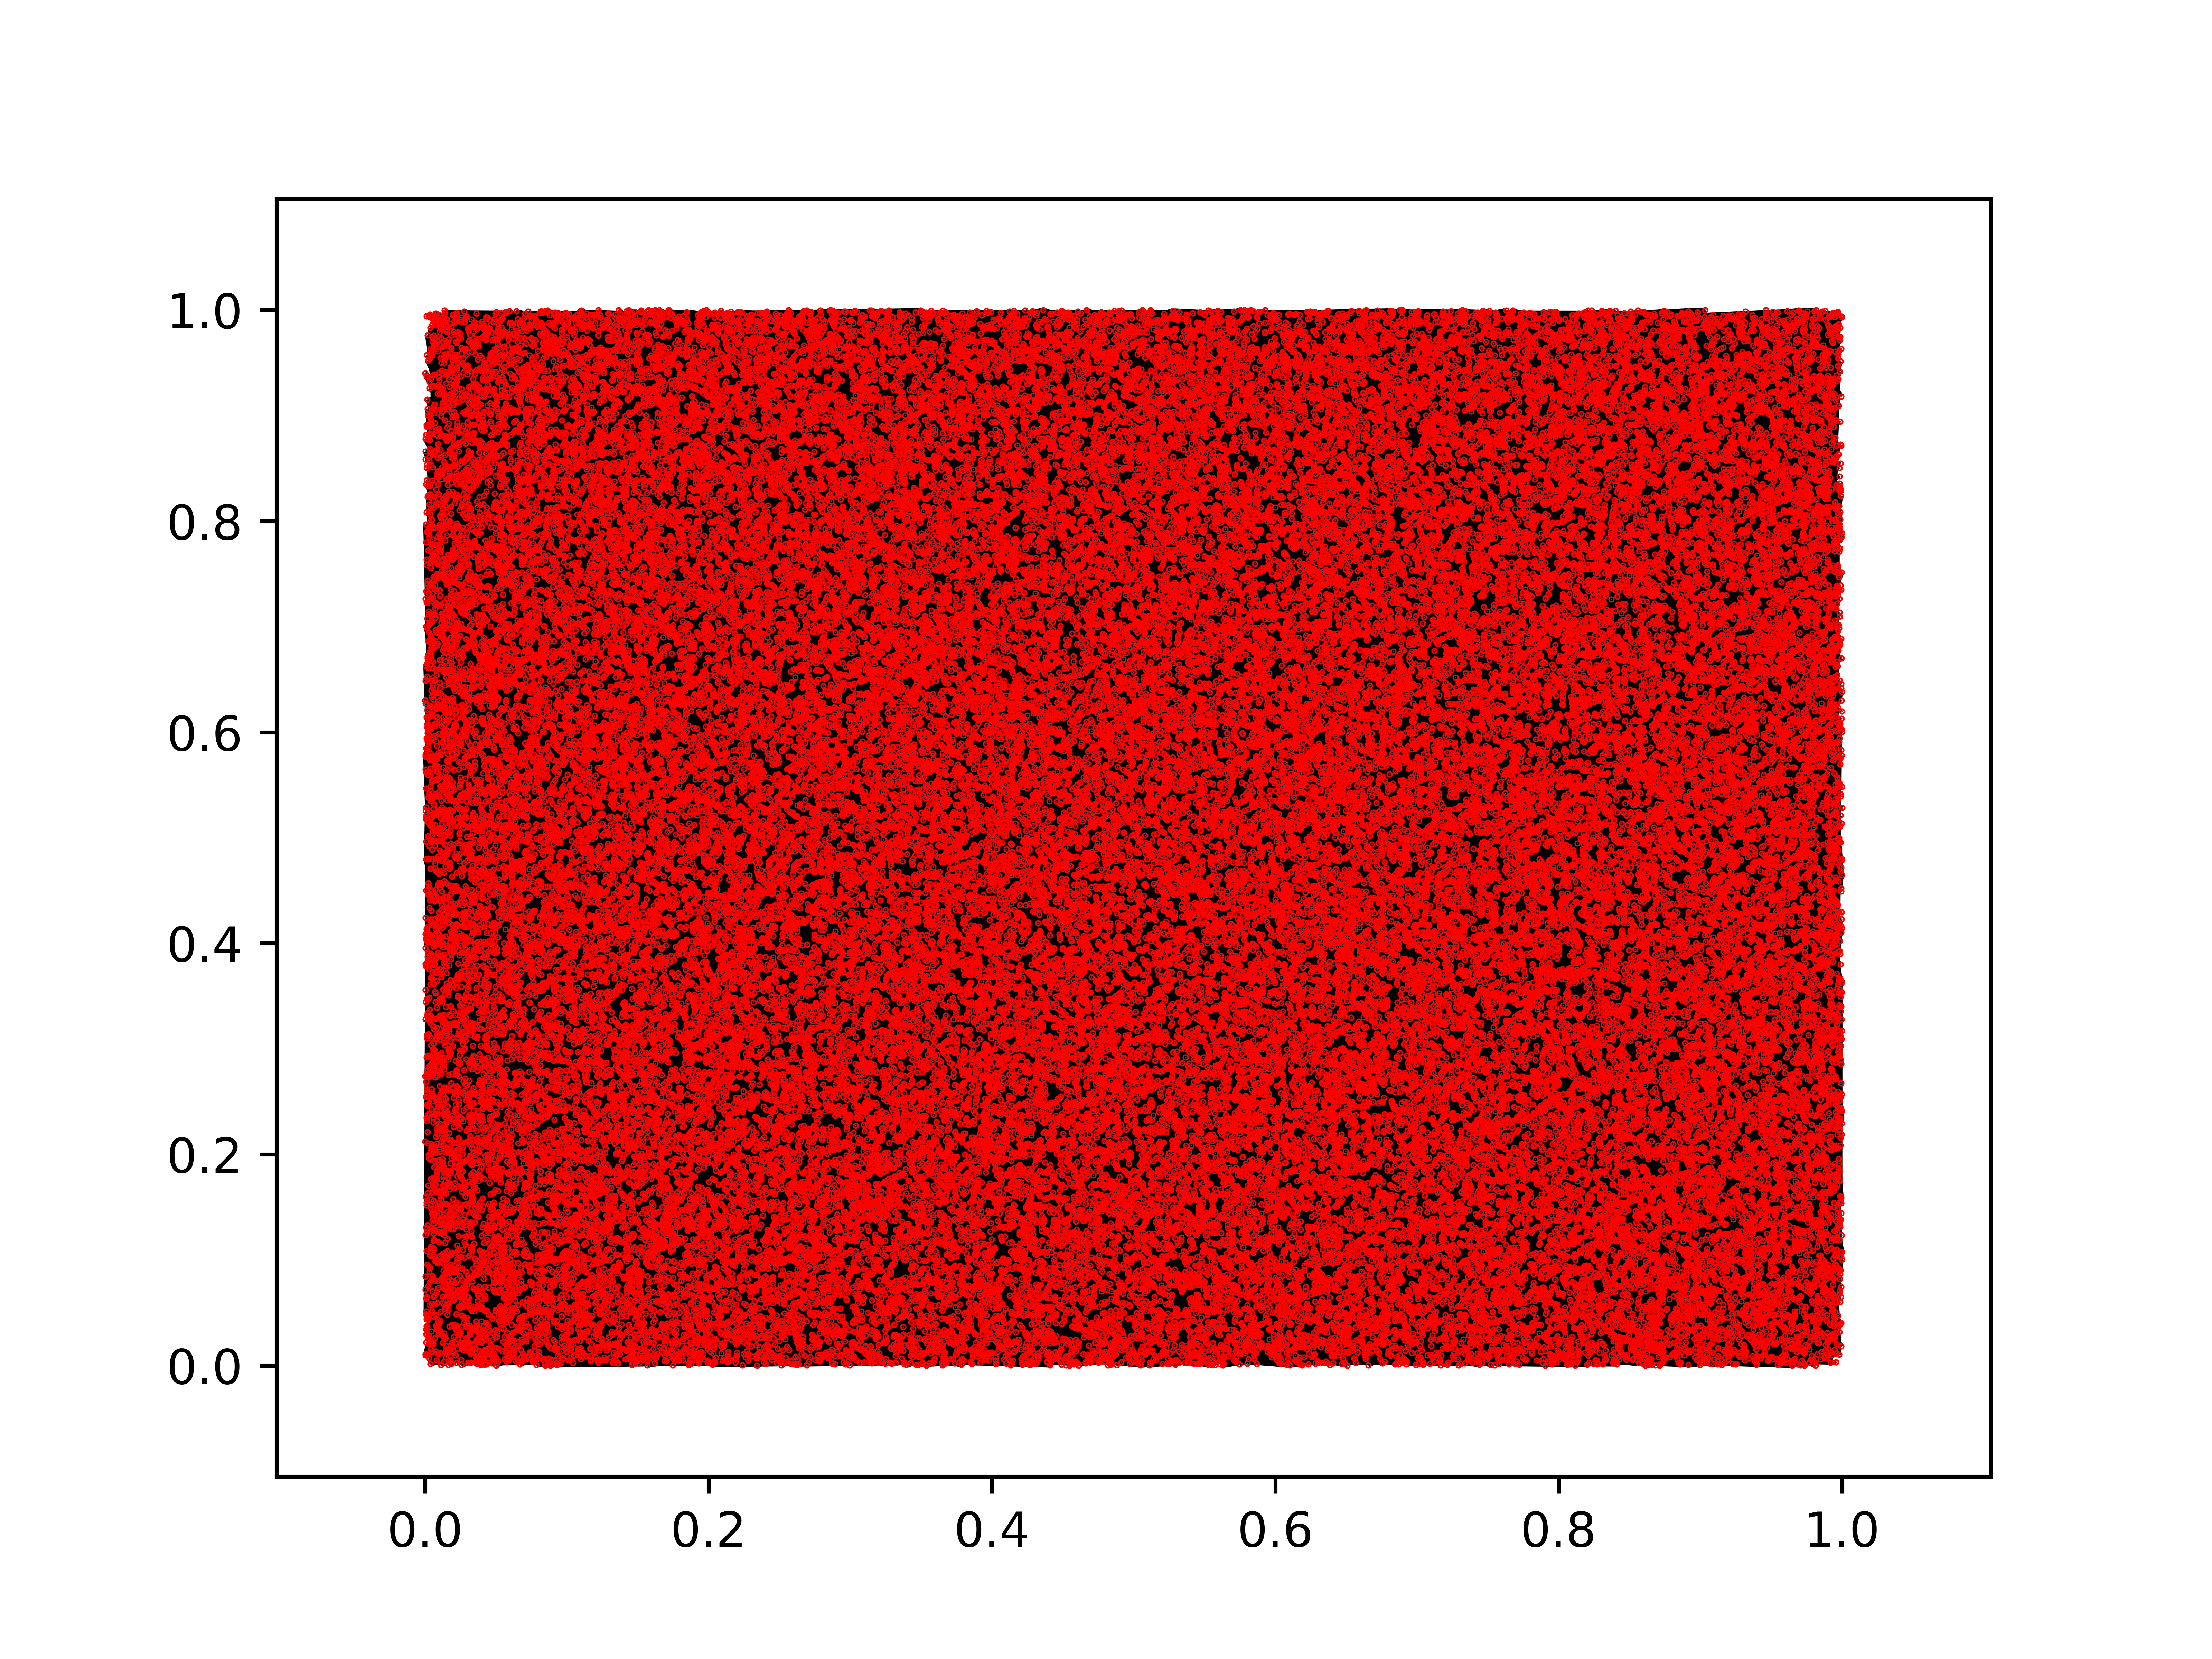
\includegraphics[width=0.75\textwidth]{NormalImgurGraph.png}
    \caption{The Fully plotted Graph of our Proposed approach.}
    \label{vofNormal}
\end{figure}

We broke down the images for 2017-10-29 to show this. Figure \ref{1post} shows how the graph looks after just a single image. The OP can be seen in the bottom left corner, as it receives edges from all users. It is most likely that the other nodes with large degree are the top commenters on the image. However, these too could point to controversial comments which could provoke other users to reply over a neutral top comment. 

\begin{figure}[h!]
    \centering
    \includegraphics[width=0.75\textwidth]{NormalImgurGraph1.png}
    \caption{One image plotted in the Graph}
    \label{1post}
\end{figure}


\par The rest of the construction of the days graph can be observed in figure \ref{545post}. Even after 1 day, the graph becomes crowded quickly.

\begin{figure}[h!]
    \centering
    \includegraphics[width=0.3\textwidth]{NormalImgurGraph5.png}
    \includegraphics[width=0.3\textwidth]{NormalImgurGraph10.png}
    \includegraphics[width=0.3\textwidth]{NormalImgurGraph15.png}
    \includegraphics[width=0.3\textwidth]{NormalImgurGraph20.png}
    \includegraphics[width=0.3\textwidth]{NormalImgurGraph25.png}
    \includegraphics[width=0.3\textwidth]{NormalImgurGraph30.png}
    \includegraphics[width=0.3\textwidth]{NormalImgurGraph35.png}
    \includegraphics[width=0.3\textwidth]{NormalImgurGraph40.png}
    \includegraphics[width=0.3\textwidth]{NormalImgurGraph45.png}
    \caption{The progression of adding nodes from images.}
    \label{545post}
\end{figure}

\par The obvious large degree nodes in our proposed approach are the OPs. We wanted to see how the graph would be affected without these large nodes, which led us to create a graph without them.

\subsection{Graph without OPs}
\par The analyzation of the graph without the OPs can be seen in table \ref{table:2}. 
\begin{table}
\centering
 \begin{tabular}{||c c c c c||} 
 \hline
 \# Nodes & \# Edges & Avg. Clustering Coef. & Connected? & Diameter \\ [0.5ex] 
 \hline\hline
 77,428 & 78,960 & 0.00519 & No & N/A \\ 
 \hline
\end{tabular} 
\caption{Analysis of graph without OPs.}
\label{table:2}
\end{table}

As seen, the number of nodes drops by 639. While one might expect the nodes to drop by 1,073 (the number of image posted), it appears that over 400 of those OPs also commented on another image, and thought they lose the edges, they do remain in the graph. Without OPs, the number of edges drops by over 200,000. This seriously hinders the graph, as the average clustering coefficient drops by ~21.5\%. The connection of the graph is also removed without OPs. This demonstrates the strength of OPs, as without them, the Imgur community becomes fractured.  
\par The full graph without OPs can be visualized in figure \ref{vofnoOPs}. Again, even with over 200,000 edges removed, the graph has too much information packed in to be useful from the very top. 
\begin{figure}[h!]
    \centering
    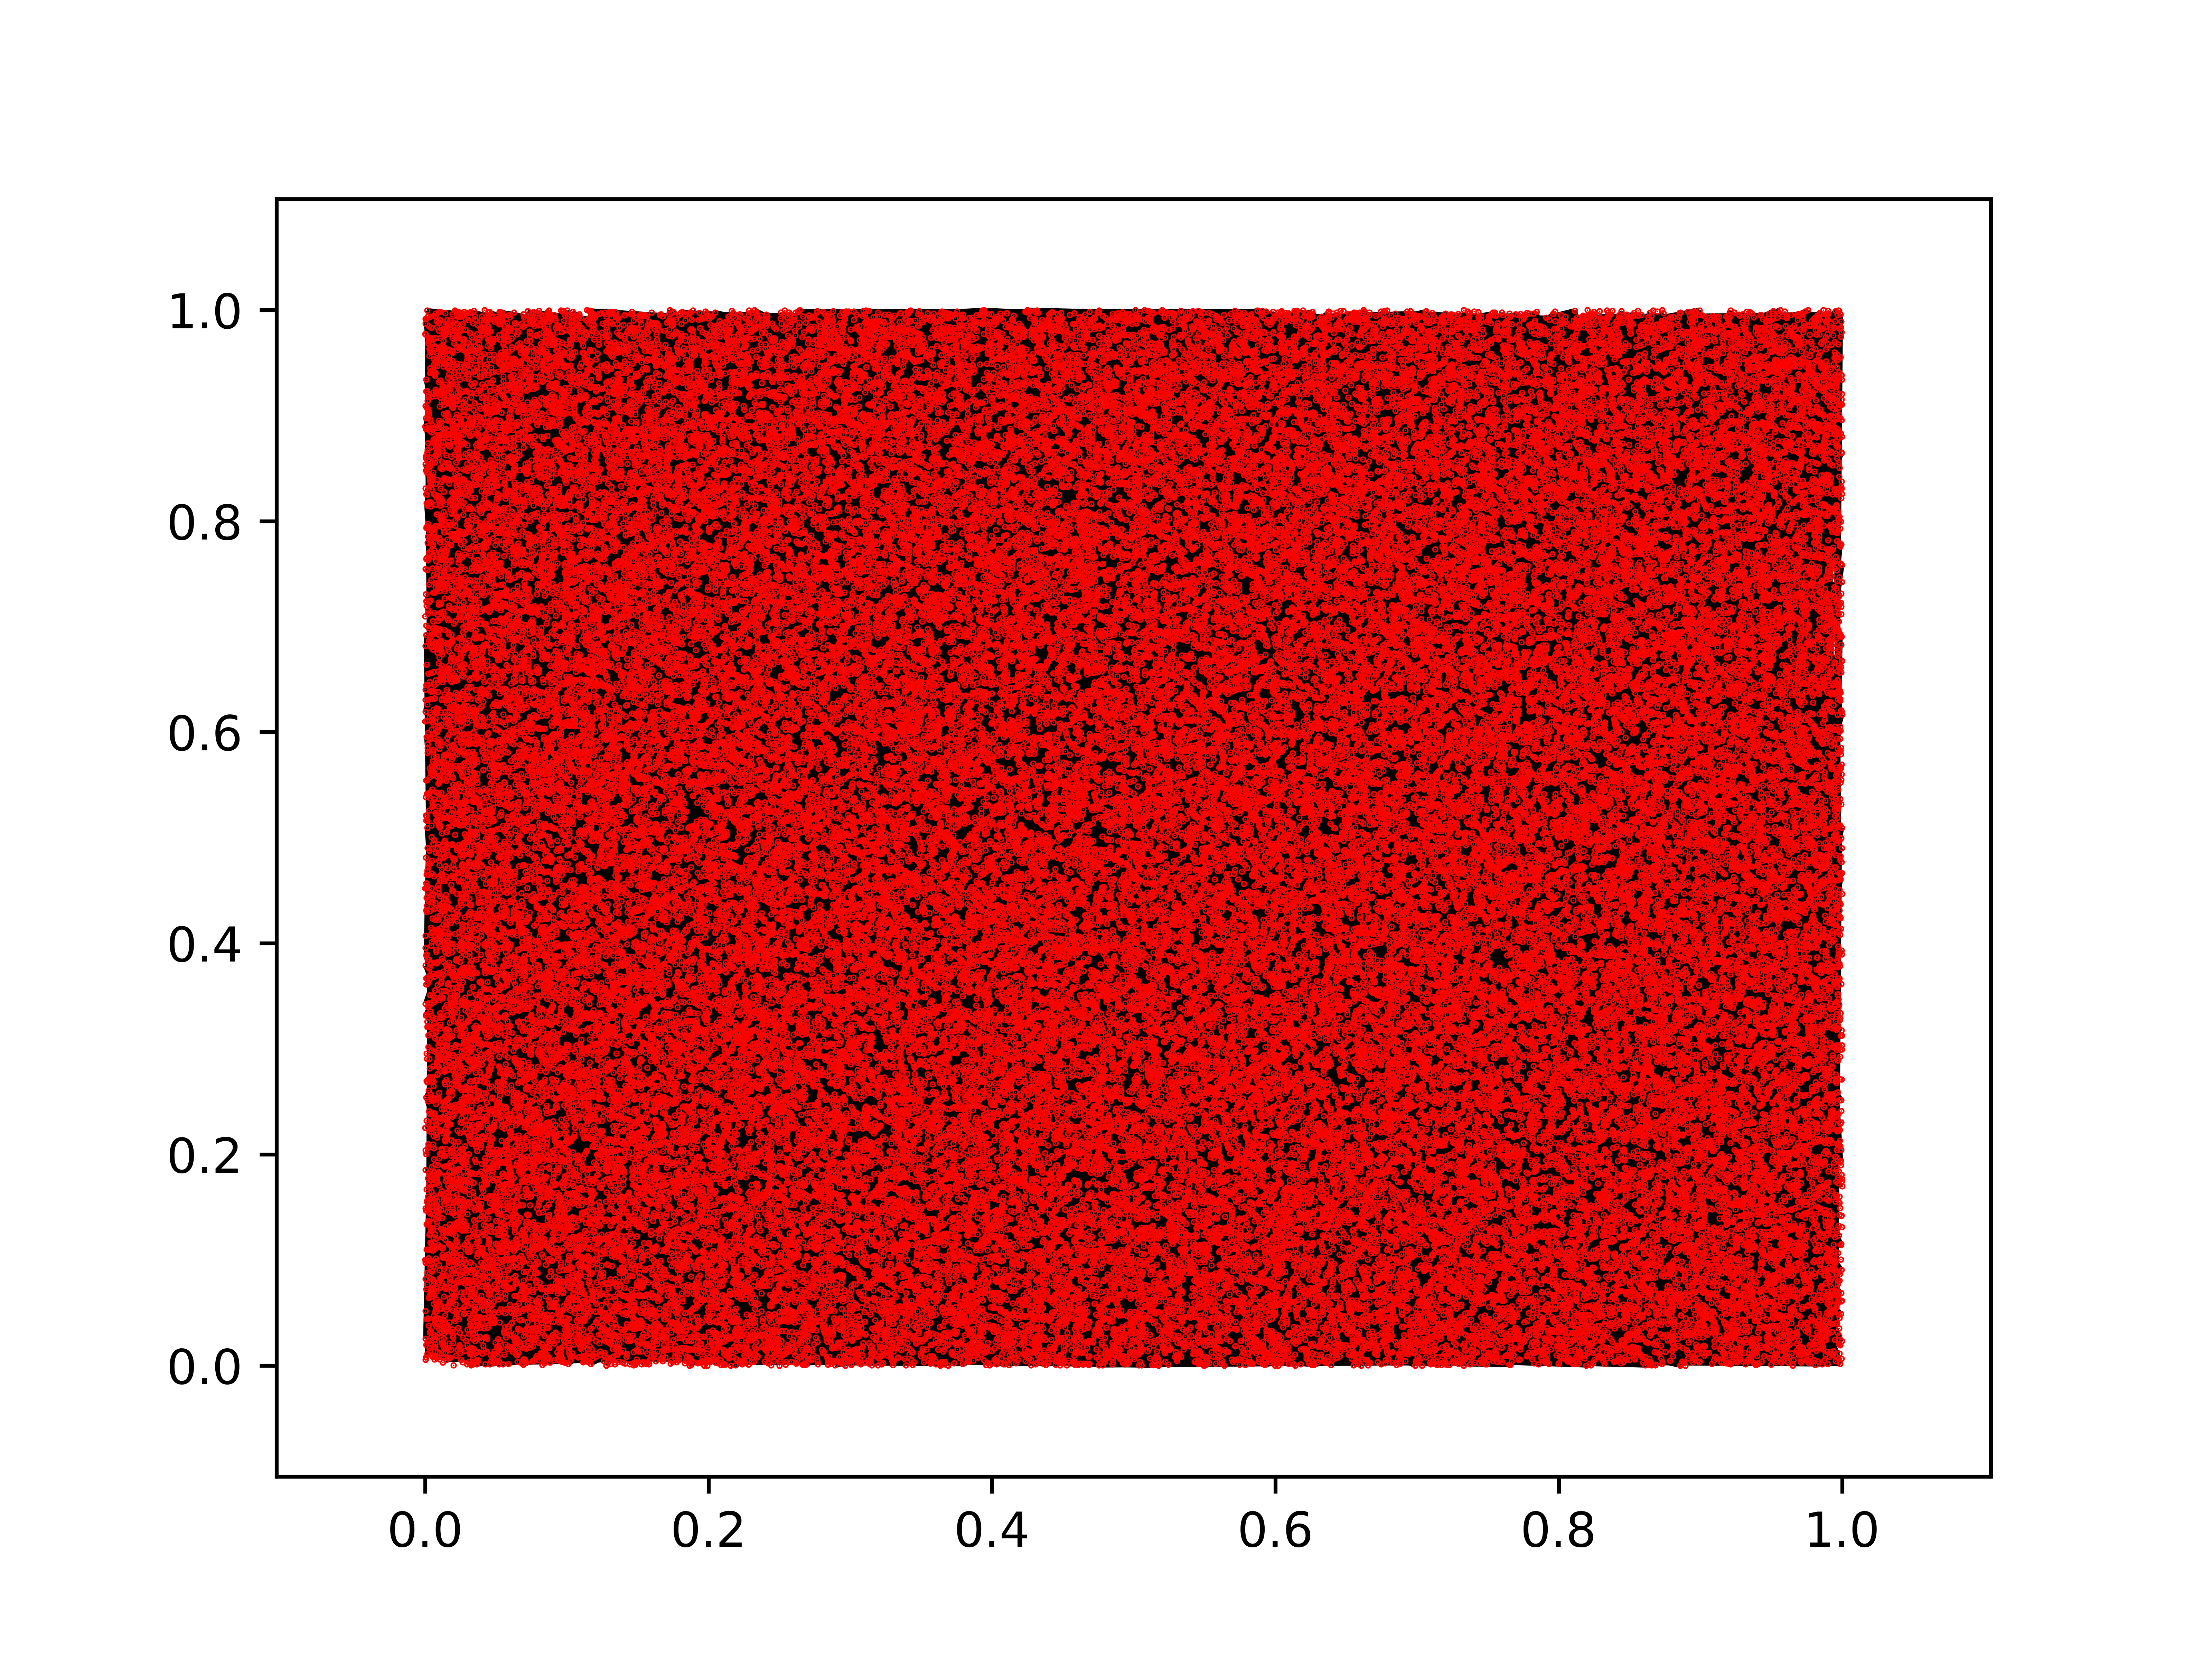
\includegraphics[width=0.75\textwidth]{NormalImgurGraphNoOp.png}
    \caption{The Fully plotted Graph without any OPs.}
    \label{vofnoOPs}
\end{figure}

We observe how the graph is constructed in one day, choosing 2017-10-29 to mirror the proposed graph. Figure \ref{post1NoOp} shows the graph after only a single image. Unlike the proposed graph, many nodes can be seen as disconnected from the rest. Now the high degree nodes become top comments on the image, as well as controversial comments. 

\begin{figure}[h!]
    \centering
    \includegraphics[width=0.75\textwidth]{NormalImgurGraphNoOp1.png}
    \caption{One image plotted in the Graph without OPs}
    \label{post1NoOp}
\end{figure}


The rest of the graph formation for that day can be observed in figure \ref{545postNoOp}. Even though the graph becomes dense, disconnected nodes can still be observed at the end of the first day, compared to the graph with OPs. 

\begin{figure}[h!]
    \centering
    \includegraphics[width=0.3\textwidth]{NormalImgurGraphNoOp5.png}
    \includegraphics[width=0.3\textwidth]{NormalImgurGraphNoOp10.png}
    \includegraphics[width=0.3\textwidth]{NormalImgurGraphNoOp15.png}
    \includegraphics[width=0.3\textwidth]{NormalImgurGraphNoOp20.png}
    \includegraphics[width=0.3\textwidth]{NormalImgurGraphNoOp25.png}
    \includegraphics[width=0.3\textwidth]{NormalImgurGraphNoOp30.png}
    \includegraphics[width=0.3\textwidth]{NormalImgurGraphNoOp35.png}
    \includegraphics[width=0.3\textwidth]{NormalImgurGraphNoOp40.png}
    \includegraphics[width=0.3\textwidth]{NormalImgurGraphNoOp45.png}
    \caption{The progression of adding nodes from images.}
    \label{545postNoOp}
\end{figure}

\par A third graph that was thought that would show interesting results was a directed graph, in which the nodes which are replied to are the in degrees, and the node replying are the out-degrees. 

\subsection{Directed Graph}
\par The directed graph has the same number of nodes and edges as the proposed graph, while the average clustering coefficient is not applicable which is why we choose to graph the directed graph, with possible future work focused on analysis. The 2017-10-29 single image post can be seen in figure \ref{post1Directed}. Similar to the proposed graph, the OP can be seen as having a large in-degree and a smaller out-degree, while the top comments again will have the higher out-degree among the comments. 

\begin{figure}[h!]
    \centering
    \includegraphics[width=0.75\textwidth]{DirectedImgurGraph1.png}
    \caption{One image plotted in the directed graph.}
    \label{post1Directed}
\end{figure}

The rest of the graph formation for the day can be observed in figure \ref{post545Directed}.

\begin{figure}[h!]
    \centering
    \includegraphics[width=0.3\textwidth]{DirectedImgurGraph5.png}
    \includegraphics[width=0.3\textwidth]{DirectedImgurGraph10.png}
    \includegraphics[width=0.3\textwidth]{DirectedImgurGraph15.png}
    \includegraphics[width=0.3\textwidth]{DirectedImgurGraph20.png}
    \includegraphics[width=0.3\textwidth]{DirectedImgurGraph25.png}
    \includegraphics[width=0.3\textwidth]{DirectedImgurGraph30.png}
    \includegraphics[width=0.3\textwidth]{DirectedImgurGraph35.png}
    \includegraphics[width=0.3\textwidth]{DirectedImgurGraph40.png}
    \includegraphics[width=0.3\textwidth]{DirectedImgurGraph45.png}
    \caption{The progression of adding nodes from images on a directed graph.}
    \label{post545Directed}
\end{figure}


\section{Conclusions}
\par To graph the Imgur community, we have collected 1,073 unique images over a 22 day period, and obtained 78,067 unique users from these images. After analyzing the graph, we can try and answer our initial question of the social of Imgur.

\subsection{How Social is Imgur?}
\par To get a sense of how social Imgur is, we compare it to Facebook from a 2011 paper which analyzed Facebook\cite{DBLP:journals/corr/abs-1111-4503}. Before we compare, we do note that we are comparing ~80,000 users to millions of users. From the paper, in May 2011, Facebook had an average user distance of 4.7. Our graph has a diameter of 6, which means that is the max two users are from each other. It can be observed then that the average user distance on Imgur would be much smaller than that of Facebook. Next, the clustering coefficient, according to the paper, for a user with 100 friends has a clustering coefficient of ~.14. Imgur has an average clustering coefficient of 0.221, showing the surprising strength of the Imgur community, even though no traditional forms of social media connections appear. 

\subsection{Future Work}
\par While we created a good basis for the graph of the Imgur community, many questions are still left to be explored. The first, is a more in depth analysis of how the graph measures up to a power law distribution. Next, a community detection algorithm through clustering and the types of images users are connected to, might show some hidden sub-communities within Imgur. A third, revolves around the fact that the graph we built was obtained from the frontpage/gallery, while other areas exist including Usersub (where user's submit images and images have a low number of votes) and Usersub rising (images have higher votes, but haven't yet achieved enough to make it to the frontpage). Graphing these other areas of Imgur then seeing how they connect to our graph could help show a broader picture of the community. Finally, 
our method view all connections throughout the 22 day period, while a temporal approach might help measure the strength of ties between users and graph a more accurate community graph. 

\medskip
\bibliographystyle{unsrt}
\bibliography{imgur}

\end{document}
